% ============================================================
%  深圳大学实验报告（Project 1：用 NumPy 复现 ViT-B/32 图像编码器）
%  编译方式：XeLaTeX（Overleaf 中 Menu -> Compiler -> XeLaTeX）
% ============================================================

\documentclass[a4paper,12pt]{article}

% ----------------------------
% 中文与字体支持
% ----------------------------
\usepackage{fontspec}
\usepackage{xeCJK}
\setCJKmainfont{Noto Serif CJK SC}

% ----------------------------
% 页面设置与常用宏包
% ----------------------------
\usepackage{geometry}
\geometry{left=1in, right=1in, top=1in, bottom=1in}

\usepackage{longtable}
\usepackage{graphicx}
\usepackage{fancyhdr}
\usepackage{tikz}
\usetikzlibrary{calc}
\usepackage{verbatim}
\usepackage{float}
\usepackage{xcolor}
\usepackage{amsmath}

% 本次自己完成的部分统一用红色标出
\newcommand{\mine}[1]{\textcolor{red}{#1}}

% ----------------------------
% 页眉页脚设置
% ----------------------------
\fancyhf{}
\fancyhead[C]{}
\fancyhead[R]{}

% ============================================================
%                      文档开始
% ============================================================

\begin{document}

% ============================================================
% 封面页
% ============================================================
\begin{titlepage}
    \centering
    \vspace*{2cm}
    \Huge{\textbf{深 \ 圳 \ 大 \ 学 \ 实 \ 验  \ 报 \ 告}}\\[1.5cm]

    {\Large\textbf{课程名称}\quad\underline{\makebox[8cm][c]{Python程序设计}}}\\[0.5cm]
{\Large
\noindent\makebox[3.2cm][l]{\textbf{项目名称}}
\underline{\makebox[8cm][c]{\small 复现 ViT-B/32 图像编码器}}}\\[0.5cm]
{\Large
\noindent\makebox[3.2cm][l]{\textbf{学 \quad \quad 院}}
\underline{\makebox[8cm][c]{人工智能学院}}}\\[0.5cm]
{\Large
\noindent\makebox[3.2cm][l]{\textbf{专 \quad \quad 业}}
\underline{\makebox[8cm][c]{}}}\\[0.5cm]
{\Large
\noindent\makebox[3.2cm][l]{\textbf{指导教师}}
\underline{\makebox[8cm][c]{舒婷}}}\\[0.5cm]
{\Large
\noindent\makebox[3.2cm][l]{\textbf{报 \quad 告 \quad 人}}
\underline{\makebox[3cm][c]{}}
\hspace{0.5cm}
\textbf{学号}
\underline{\makebox[3cm][c]{}}}\\[0.5cm]
{\Large
\noindent\makebox[3.2cm][l]{\textbf{实验时间}}
\underline{\makebox[8cm][c]{}}}\\[0.5cm]
{\Large
\noindent\makebox[3.2cm][l]{\textbf{提交时间}}
\underline{\makebox[8cm][c]{}}}\\[1.5cm]

    \vfill
    \Large{\textbf{教务处制}}
\end{titlepage}

\newpage

% ============================================================
% 正文部分
% ============================================================

\section{Objectives}

本实验的目标是\textbf{只用 NumPy} 复现 CLIP 视觉塔（OpenCLIP \texttt{ViT-B/32}）的完整前向计算：
输入是预处理后的图像张量 $[B,3,224,224]$ 与课程提供的 152 个 float32 参数张量，输出是每张图一个
$[B,512]$ 的单位化 token。全程不涉及任何参数训练，权重来自固定 checkpoint，因此“对”的唯一标准就是
与参考 FP32 结果在给定容差内一致。

需要自己完成的是 6 个 TODO，分别落在切块、多头拆分、注意力、Transformer 块、嵌入和最终输出上。
除跑通之外，实验还要求说明三件事：各中间阶段的数值误差有多大、误差从何而来；一处关键形状变换
为什么必须那样写；以及一个真正踩到的 bug 及其修复过程。

\section{Overview}

整体思路是“先把一张图变成一串 token，再让这串 token 互相看 12 轮，最后从汇总位读出结果”，
数据流与形状变化如图~\ref{fig:pipeline}。

\begin{figure}[H]
  \centering
  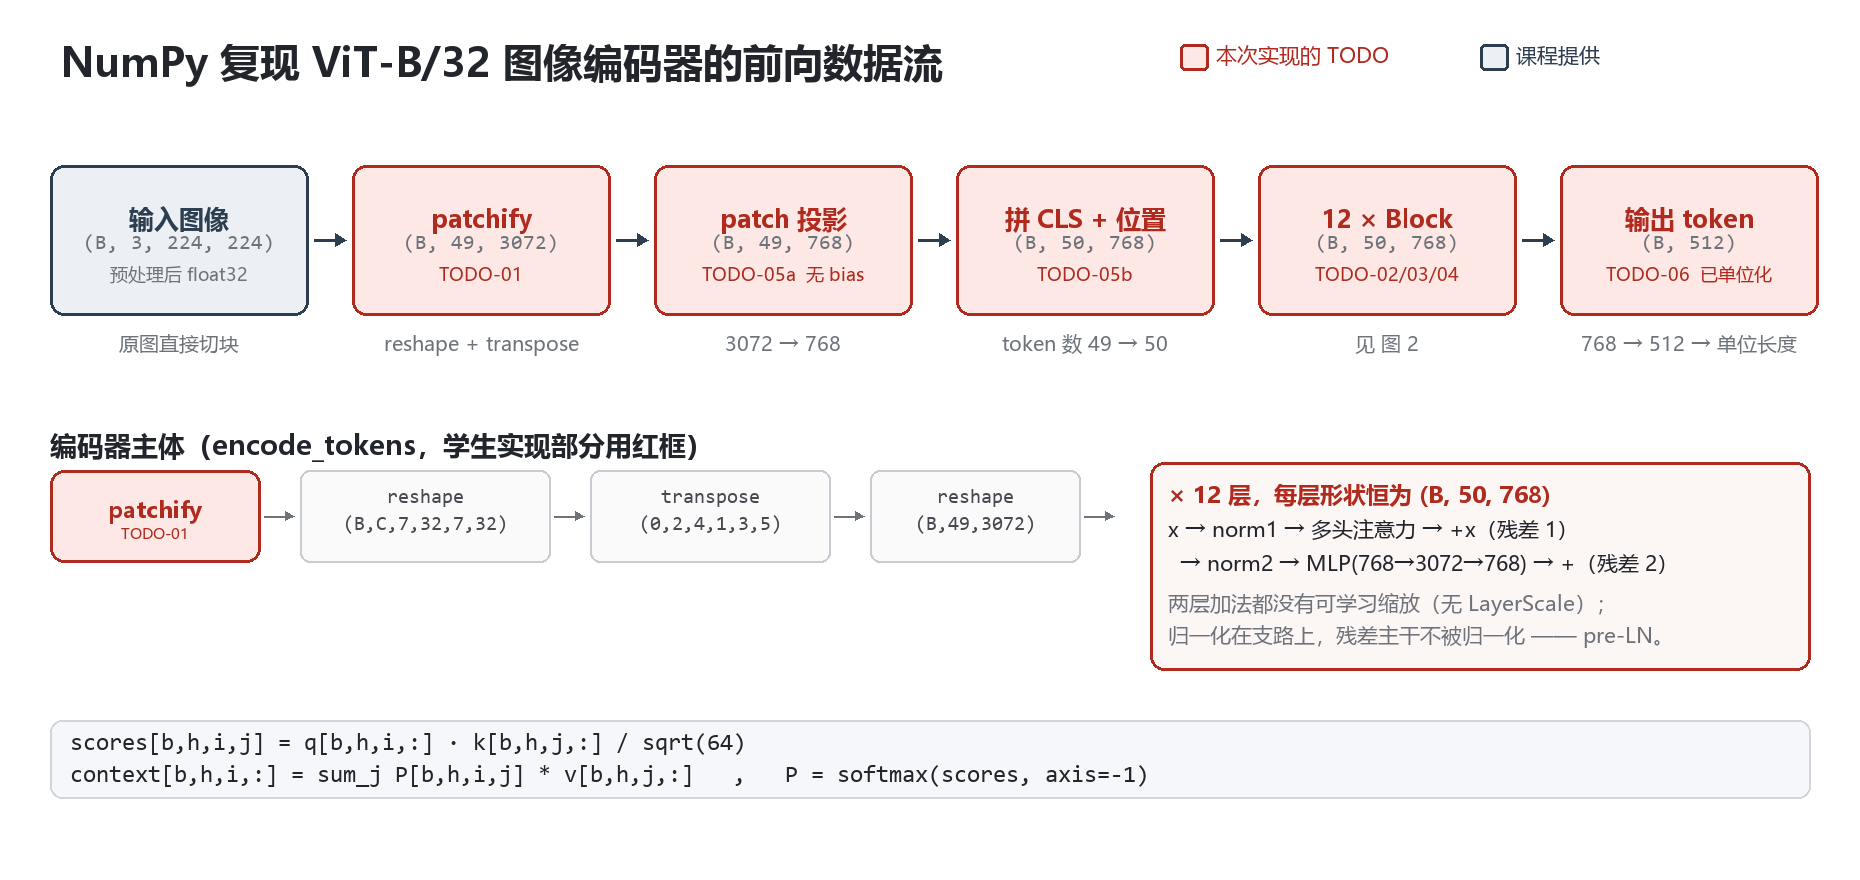
\includegraphics[width=\linewidth]{figs/pipeline.png}
  \caption{ViT-B/32 图像编码器的前向数据流。红框为本次实现的 6 个 TODO，蓝框为课程提供的固定参数或辅助函数。}
  \label{fig:pipeline}
\end{figure}

实现分四个阶段：

\begin{enumerate}
  \item[阶段一] 切块与嵌入：$[B,3,224,224]\to[B,49,3072]\to[B,49,768]$，再前置 CLS 并加上位置编码，
        得到 $[B,50,768]$；
  \item[阶段二] 编码：12 个结构相同的 Transformer 块，每块一次多头注意力、一次 MLP，各自带残差加法，
        形状自始至终保持 $[B,50,768]$；
  \item[阶段三] 读出：取第 0 行（CLS），经 post-norm 与 $768\times512$ 投影压到 512 维；
  \item[阶段四] 归一化：单位化，使输出之间的点积等于余弦相似度。
\end{enumerate}

工程上坚持三条做法。第一，\mine{只修改 \texttt{image\_encoder.py}}：预处理、\texttt{LayerNorm}、
精确 GELU、softmax、权重和参考数据一律不动，保证比较的是“我的前向”而不是“我改了题目”。
第二，\mine{逐关验证}：\texttt{check.py} 把前向切成 8 个可独立比较的阶段，哪一关先红就说明错误
落在哪一段，避免在 12 层里盲试。第三，\mine{形状先行}：每个 TODO 先写出输入输出形状再动手，
形状对不上时错误立刻暴露，而不是等到数值检查报 $10^{-1}$ 量级的误差才发现。

\section{Implementations}

一个 Transformer 块的内部结构，以及多头注意力中 q/k/v 的产生与合并方式，见图~\ref{fig:block}；
表~\ref{tab:todo} 汇总 6 个 TODO 的实现要点，随后逐条说明。

\begin{figure}[H]
  \centering
  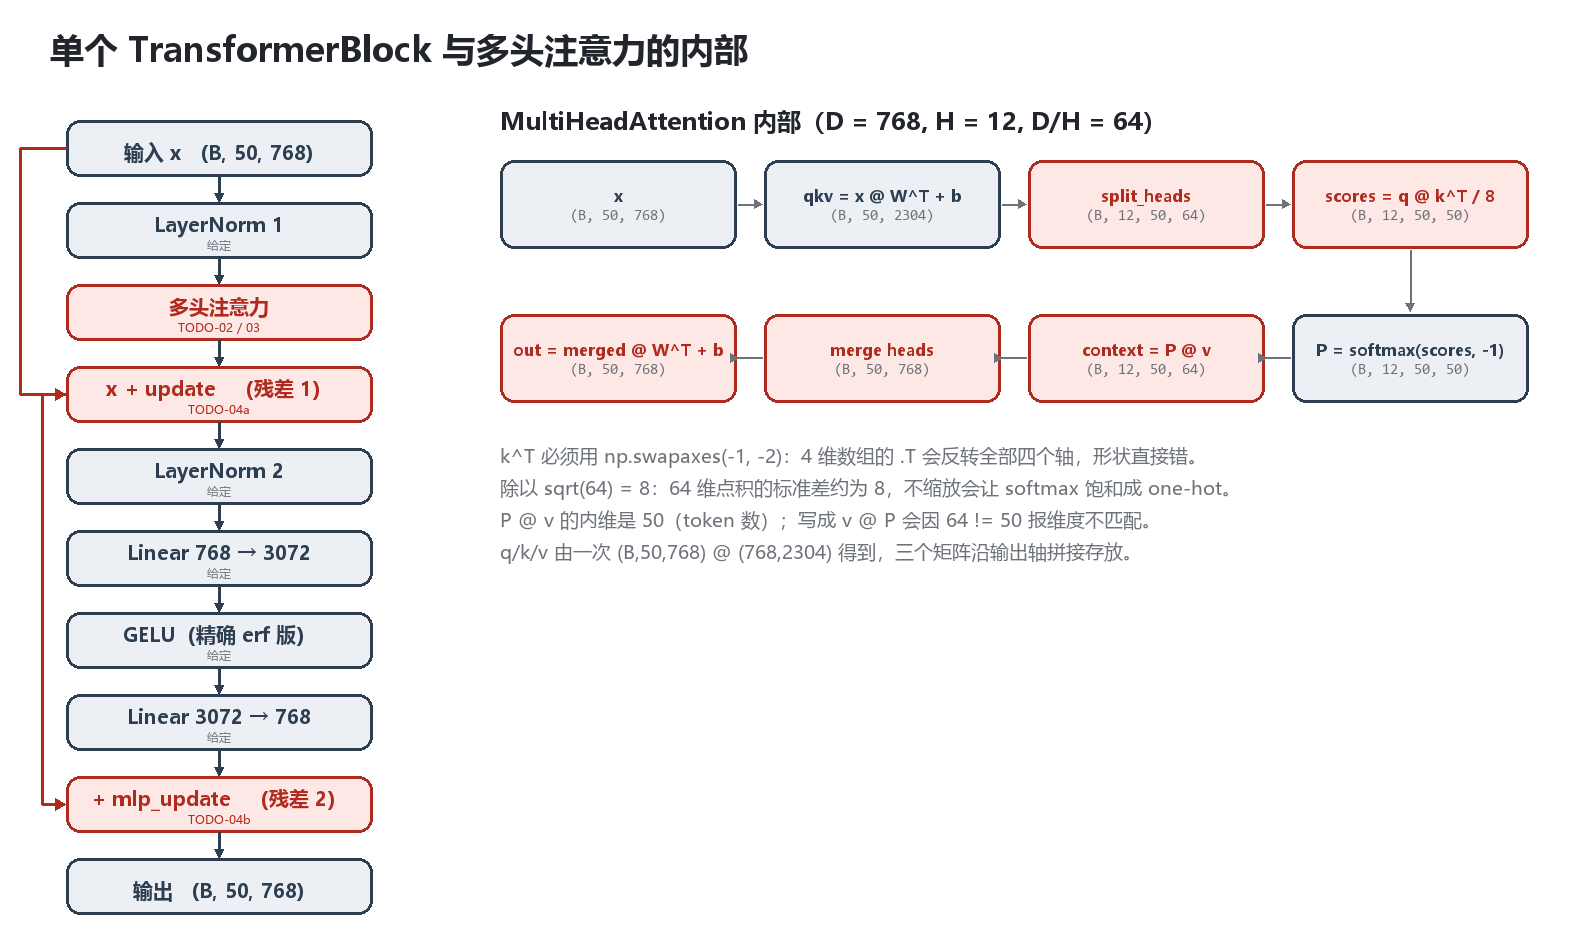
\includegraphics[width=0.86\linewidth]{figs/block.png}
  \caption{左：单个 Transformer 块，pre-LN 结构与两处残差加法。右：多头注意力内部，q/k/v 由一次
  融合矩阵乘法得到，12 个头独立计算后合并再做输出投影。}
  \label{fig:block}
\end{figure}

\begin{table}[H]
\centering\small
\caption{六个 TODO 的实现要点（关键行以红色标出）}
\label{tab:todo}
\begin{tabular}{@{}llp{8.0cm}l@{}}
\hline
TODO & 方法 & 关键实现 & 输出形状 \\
\hline
01 & \texttt{patchify} & \mine{六轴 reshape 成 $(B,C,7,32,7,32)$，转置 $(0,2,4,1,3,5)$ 后再 reshape} & $(B,49,3072)$ \\
02 & \texttt{split\_heads} & \mine{reshape 成 $(B,N,H,D/H)$，再把 head 轴换到批次位} & $(B,12,50,64)$ \\
03 & \texttt{\_\_call\_\_} & \mine{$q k^{\top}/\sqrt{64}$、$\mathrm{softmax}$ 加权、合并头、输出投影} & $(B,50,768)$ \\
04 & \texttt{\_\_call\_\_} & \mine{两条 pre-LN 残差；MLP 为 $768\to3072\to768$} & $(B,50,768)$ \\
05 & \texttt{embed} & \mine{无 bias 投影；CLS 拼在 token 轴（axis=1）；广播加位置} & $(B,50,768)$ \\
06 & \texttt{\_\_call\_\_} & \mine{取 CLS、post-norm、$768\to512$ 投影，最后单位化} & $(B,512)$ \\
\hline
\end{tabular}
\end{table}

\begin{enumerate}

\item[TODO-01] 切块的关键不是“切”，而是\textbf{切完之后的摊平顺序}。224 本来就是 $7\times32$，
所以先把 $(B,3,224,224)$ reshape 成 $(B,3,7,32,7,32)$，再转置成 $(B,7,7,3,32,32)$，让
(grid\_row, grid\_col) 变成 49 个 token 的两个轴、$(3,32,32)$ 变成一个 token 的 3072 个特征。
\mine{顺序必须是 C$\to$H$\to$W}，因为参数里 \texttt{visual.conv1.weight} 的形状是 $(768,3,32,32)$，
被 reshape 成 $(768,3072)$ 时正是按这个顺序摊平的；两边顺序不一致时形状照样对得上，但每个滤波器的
权重会与像素错配，误差直接到 $10^{-1}$ 量级。

\item[TODO-02] 多头拆分是两次纯搬运：先把 768 维切成 12 个连续的 64 维小段（reshape），再把 head
轴提到 token 轴前面（transpose），得到 $(B,12,50,64)$。\mine{head 必须待在批次位上}，因为后面
$q k^{\top}$ 只对最后两维做矩阵乘、其余维当批次，这样一次就能算完 12 个头互不干扰的注意力矩阵。

\item[TODO-03] 注意力分四步：打分、归一化、加权、投影。打分用 $q k^{\top}/\sqrt{64}$，其中
\mine{$k$ 的转置必须用 \texttt{np.swapaxes(k,-1,-2)}}而不写成 \texttt{k.T}（见第 \ref{sec:bug} 节）；
除以 $\sqrt{64}=8$ 是因为 64 维点积的标准差约为 8，不缩放会让 softmax 饱和成 one-hot、梯度消失。
\texttt{attention\_weights} 沿最后一轴做 softmax，得到每行和为 1 的系数矩阵；再用
$\mathrm{coefficients}\ @\ v$ 对 50 个 value 行做加权平均，\mine{内维是 token 数 50}。合并头是
拆分的逆操作（转置回 $(B,N,H,64)$ 再 reshape 成 $(B,N,768)$），最后过一次输出投影，让 12 个头的结果
互相混合。

\item[TODO-04] 一个块里有两处残差，\mine{加回的都是残差主干上的 $x$，而不是归一化之后的值}，
这是 pre-LN 结构与原版 Transformer 的核心区别：归一化在支路上，主干是一条不被缩放的高速通路，
12 层才能稳定训练。MLP 部分先把 768 维升到 3072 维，过精确 erf 版 GELU，再降回 768 维；
OpenCLIP 的 ViT-B/32 \mine{没有 LayerScale 参数}，所以残差不能乘任何可学习缩放。

\item[TODO-05] 投影是 $(B,49,3072)\times(3072,768)$，\mine{没有 bias}（参数里根本没有
\texttt{visual.conv1.bias}，等价于 \texttt{Conv2d(bias=False)}）。CLS 用 \texttt{np.tile} 复制成
$(B,1,768)$ 后与 patch token 在第 1 轴拼接，\mine{axis=1 才是 token 轴}：写成 axis=0 会变成
$(2B,49,768)$，写成 axis=2 会变成 $(B,49,1536)$。最后加 $(50,768)$ 的位置编码，靠广播复制 B 份。
位置编码是必需的，因为注意力本身置换不变，不加位置信息模型无法区分 patch 的左右上下。

\item[TODO-06] 取第 0 行即 CLS——它在 12 层里通过注意力看过所有 patch，是一个学出来的摘要。
之后 post-norm 对 768 维重新归一化，投影到 512 维，最后单位化。
\mine{投影矩阵不能转置}：参数里的 \texttt{visual.proj} 已经是 $[in,out]=(768,512)$，与其他以
$[out,in]$ 存储的线性层不同，加了 \texttt{.T} 会直接报内维 768 与 512 不匹配。

\end{enumerate}

\section{Results}

\subsection*{4.1 逐阶段数值检查}

按 \texttt{check.py} 的 8 个阶段逐一比较，结果全部通过（表~\ref{tab:err}）。容差为
$\lvert \text{actual}-\text{reference}\rvert \le atol + rtol\lvert\text{reference}\rvert$。

\begin{table}[H]
\centering\small
\caption{各阶段与参考实现的最大与平均绝对误差}
\label{tab:err}
\begin{tabular}{@{}lcrrrl@{}}
\hline
阶段 & 输出形状 & max\_abs & mean\_abs & 容差 & 结论 \\
\hline
assets      & —              & —          & —          & —      & 152 个张量与 10 组图像匹配 \\
preprocess  & $(10,3,224,224)$ & 0          & 0          & $2\times10^{-6}$ & PASS \\
patches     & $(2,49,3072)$  & 0          & 0          & $2\times10^{-4}$ & PASS \\
tokens      & $(2,50,768)$   & $4.005\times10^{-5}$ & $1.289\times10^{-6}$ & $2\times10^{-4}$ & PASS \\
block0      & $(2,50,768)$   & $7.063\times10^{-6}$ & $3.250\times10^{-7}$ & $2\times10^{-4}$ & PASS \\
last\_tokens & $(2,50,768)$  & $4.768\times10^{-5}$ & $2.696\times10^{-6}$ & $2\times10^{-4}$ & PASS \\
output      & $(10,512)$     & $5.439\times10^{-7}$ & $8.311\times10^{-8}$ & $2\times10^{-5}$ & PASS \\
batch       & $(3,512)$      & $4.619\times10^{-7}$ & $7.632\times10^{-8}$ & $2\times10^{-5}$ & PASS \\
\hline
\end{tabular}
\end{table}

其中 \texttt{batch} 关特意打乱图像顺序并插入重复图片，用来证明实现是真的逐张计算，
而不是返回缓存的参考行；每行的长度经验证均为 1（单位化正确）。

\subsection*{4.2 复现命令}

\begin{verbatim}
python check.py --stage all
python run.py --output output_tokens.npz
\end{verbatim}

\begin{verbatim}
output       PASS shape=(10, 512) max_abs=5.439e-07 mean_abs=8.311e-08
batch        PASS shape=(3, 512)  max_abs=4.619e-07 mean_abs=7.632e-08
Saved (10, 512) to output_tokens.npz
\end{verbatim}

\section{Discussion}

\subsection*{5.1 误差从哪来}

\texttt{preprocess} 与 \texttt{patches} 的误差严格为 0，因为这两步只有重新取数和搬运，没有任何算术，
与参考实现逐位相同。从 \texttt{tokens} 开始出现 $10^{-5}$ 量级的差异，来源是 float32 的累加顺序：
参考实现用 Torch（不同的分块与 SIMD 顺序），我们用 NumPy，同一个数学表达式在浮点上的舍入路径不同，
这不是算法错误。

一个有意思的现象是 \texttt{last\_tokens}（$4.8\times10^{-5}$）比 \texttt{block0}
（$7.1\times10^{-6}$）大了一个数量级，因为 12 层逐层累积；但 \texttt{output} 反而最小
（$5.4\times10^{-7}$）：post-norm 把数值重新标准化，单位化又把每行长度压到 1，绝对幅度变小，
绝对误差自然跟着变小。这也解释了为什么输出层的容差可以收紧到 $2\times10^{-5}$ 而不误杀。

\subsection*{5.2 一处关键形状变化}

最能说明问题的是 \texttt{patchify} 里的六轴分解。224 在原来的张量里是“一个空间轴”，经过
$(B,3,224,224)\to(B,3,7,32,7,32)$ 的 reshape，它被重新解释成“7 个块 $\times$ 每块 32”，
随后转置 $(0,2,4,1,3,5)$ 把两个网格轴提到 token 位置：

\[
(B,C,\underbrace{7}_{\text{行块}},\underbrace{32}_{\text{行内}},\underbrace{7}_{\text{列块}},\underbrace{32}_{\text{列内}})
\;\longrightarrow\;
(B,\underbrace{7,7}_{\text{49 个 token}},\underbrace{C,32,32}_{\text{3072 个特征}}).
\]

这两步本身不移动任何数据，只是改变了“怎么索引同一批数字”，最后一步 reshape 才真正把
$(7,7)$ 摊成 49、把 $(3,32,32)$ 摊成 3072。正方体没变，只是换了观察角度——这也是它误差为 0 的原因。

\subsection*{5.3 一个踩到的 bug}
\label{sec:bug}

写注意力打分时，第一版按 2 维的习惯写成了 \texttt{scores = q @ k.T}。$q$ 与 $k$ 的形状都是
$(B,12,50,64)$，而 4 维数组的 \texttt{.T} 会\textbf{反转全部四个轴}，\texttt{k.T} 变成
$(64,50,12,2)$，于是 NumPy 报：

\begin{verbatim}
ValueError: matmul: Input operand 1 has a mismatch in its core dimension 0,
with gufunc signature (n?,k),(k,m?)->(n?,m?) (size 12 is different from 64)
\end{verbatim}

报错里“size 12 is different from 64”很有迷惑性：直觉上只该关心最后两维 $(50,64)$，但 4 维数组的
\texttt{.T} 连批次轴一起反了，NumPy 只能报出第一个对不上的维度。\mine{正确写法是
\texttt{np.swapaxes(k,-1,-2)}}，它只交换最后两轴，得到 $(B,12,64,50)$，批次与 head 分组原样保留。
教训是：在 $n$ 维数组上不要用 \texttt{.T} 表达“转置最后两维”，二者的语义在多维下并不相同；
凡是“只想转置最后一对轴”的场合，都应显式写出 \texttt{swapaxes}。

\subsection*{5.4 效率与可改进之处}

当前实现最慢的一环是 \texttt{helpers.py} 里的精确 GELU：它用 Python 循环逐元素调用
\texttt{math.erf}，跑完 10 张图约需 1–2 分钟（12 层 $\times$ 50 token $\times$ 3072 $\approx$
$1.8\times10^{7}$ 次调用）。若允许修改辅助函数，可以用 \texttt{scipy.special.erf} 的向量化版本，
或用 \texttt{0.5x(1+erf(x/\sqrt2))} 的查表近似，速度可提升两个数量级，代价是与参考的误差会略微
变大（约 $10^{-7}$，仍在容差内）。

另外，多头注意力中的三次矩阵乘法可以用 \texttt{np.einsum} 合并表达，可读性更好；但当前写法与
课堂讲的“打分—归一化—加权—投影”四步一一对应，更利于逐步对照检查，因此保留。

\subsection*{5.5 个人贡献与使用的帮助}

6 个 TODO 的实现代码由本人逐行输入并逐关验证；\mine{关键判断（patch 摊平顺序、swapaxes 的正确用法、
CLS 拼接轴、投影矩阵不转置）均由本人在推导形状后确定}。课程提供的 \texttt{helpers.py}、
\texttt{preprocess\_image.py}、\texttt{check.py} 与权重未作任何修改。实现过程中参考了课堂
slides 46--76 与课程 README，并使用 AI 助手辅助理解概念、核对数值与排版绘图，所有结论均以
\texttt{check.py} 的实际输出为准。

\newpage

% ============================================================
% 批阅与成绩评定页
% ============================================================

\begin{tikzpicture}[remember picture, overlay]
  \draw[thick]
    ($(current page.north west)+(2cm,-3cm)$)
    rectangle
    ($(current page.south east)+(-2cm,3.5cm)$);
\end{tikzpicture}

\vspace{1cm}

\noindent \textbf{指导教师批阅意见：}
\vspace{6cm}
\hfill

\vspace{1cm}

\noindent \textbf{成绩评定：}
\vspace{2cm}
\hfill

\vspace{1cm}

\noindent
\hfill
\textbf{指导教师签字：}\quad\quad\quad\quad\quad\\[0.5cm]

\hfill
\textbf{年}\quad\quad
\textbf{月}\quad\quad
\textbf{日}\quad

\vspace{1cm}

\noindent \textbf{备注：}

\begin{tikzpicture}[remember picture, overlay]
  \node[
    anchor=north west,
    inner sep=0pt,
    text width=\dimexpr\paperwidth-4cm\relax
  ] at ($(current page.south west)+(2cm,3.1cm)$) {
    \begin{minipage}{\dimexpr\paperwidth-4cm\relax}
      \small
      \noindent
      \textbf{注：}\;1、报告内的项目或内容设置，可根据实际情况加以调整和补充。\\[0.2cm]
      \phantom{\textbf{注：}\;}2、教师批改学生实验报告时间应在学生提交实验报告时间后 10 日内。
    \end{minipage}
  };
\end{tikzpicture}

\end{document}
